\section{Timer}
L' ATMega32 è dotato di 3 timer interni:
\begin{itemize}
    \item timer 0
    \item timer 1
    \item timer 2
\end{itemize}
I timer 0 e 2 sono molto simili.

\subsection{Timer 0}
TCNT0 è un registro ad 8 bit, il suo valore è incrementato in maniera automatica tramite il clock o un suo derivato.
Posso scriverci un valore a piacere e leggere il valore corrente in qualsiasi momento.
Quando conta conta solo in avanti da 0 a 255, dopodiché si \emph{wrappa} e torna a 0 e così via.

\begin{figure}[H]
    \centering
    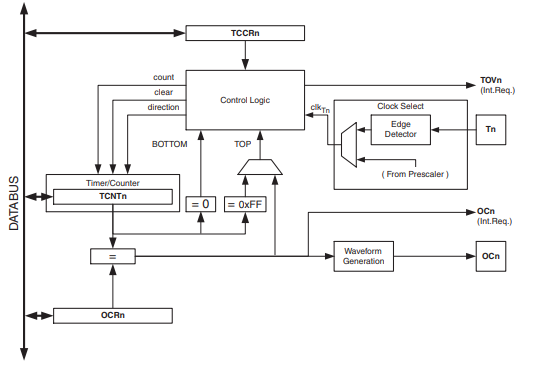
\includegraphics[width=300px]{images/18_Timer/Timer0.png}
\end{figure}

\subsubsection{Utilizzo come timer}
Incrementa il contatore ogni $\tau$ più o meno a scelta.
E' usato per misurare intervalli di tempo e se 256 valori non bastano si possono contare i wrap.
Più la frequenza è alta e più è alta la risoluzione ma più velocemente il contatore fa wrap!
Ogni volta che il contatore torna a 0 un' interruzione viene lanciata e può essere catchata per farci qualcosa.

In questa configurazione il clock è quello del processore, spesso tuttavia risulta troppo veloce, per rallentarlo possiamo usare il \emph{prescaler} integrato configurabile ai valori: 1, 8, 64, 256, 1024.

NB: il prescaler impostato ad 1 è il default ed implica che non ci sia un vero e proprio rallentamento del clock. 8, 64, ecc invece indicano che anziché aggiornare ad ogni tick del clock si aggiorna ogni 8, ogni 64, ecc, ecc.

\subsubsection{Utilizzo come contatore}
Conta gli eventi sporadici, l' aggiornamento non è periodico.
Per ottenere questa funzionalità il clock del contatore è esterno, un pin apposito del package

Per configurarlo in questo modo bisogna collegare l' ingresso esterno T0 all' ingresso del contatore.

\subsubsection{Comparatore}
All' interno della struttura del timer esiste un altro registro: OCR0, una volta asegnatogli un valore esso vi rimane, ogni volta che TCNT0 viene incrementato una rete combinatoria controlla se il valore corrente è uguale al contenuto di OCR0, se combaciano viene lanciata una interruzione.
Un utilizzo tipico è quello di contare intervalli costanti:
\begin{itemize}
    \item setto OCR0 a 70
    \item abilito il clock su TCNT0
    \item quando TCNT0 sta transitando da 70 a 0 arriva l'interrupt (ho ottenuto un \emph{match})
    \item nel gestore dell' interruzione azzero TCNT0 per fargli contare di nuovo un intervallo fisso
\end{itemize}
La stessa rete combinatoria che mi lancia l' interruzione può ripulire il registro TCNT0, quindi questo conteggio può essere eseguito in automatico.

Questo segnale di match può essere anche usato per alterare lo stato del pin di uscita OC0:
\begin{itemize}
    \item alzare OC0
    \item abbassare OC0
    \item toggle di OC0 (cioè commutare lo stato corrente)
\end{itemize}

Possiamo ad esempio generare un' onda quadra ad una certa frequenza: supponiamo di voler generare un' onda quadra a 400Hz, il periodo deve essere di $T = \frac{1}{400 Hz} = 2.5 ms = 2500 \mu s$.
Supponiamo di avere $f_{ck} = 1 MHz$ e quindi periodi di $1\mu s$, ci serve avere un match ogni $\frac{T}{2} = 1250\mu s$ cioè un match ogni 1250 cicli di clock.
% TODO disegno onda quadra con periodi %
Usando un prescaler ad 8 mi serve un match ogni $\frac{1250}{8} = 156,25$, arrotondiamo a 156, quindi in OCR0 andrò ad inserire il valore 156.
Per la precisione il match è ogni $1248\mu s$ quindi perdo $4\mu s$ ad ogni periodo.
Se usassi il prescaler a 64 in OCR0 dovrei metterci 20 ma facendo i conti il valore corretto sarebbe 19.53 quindi ho un errore sul periodo più grande. 

Il prescaler a valori alti serve per $f_{ck}$ alto o per periodi lunghi.

Es: $f = 30KHz$, $T = 33\mu s$, $\frac{T}{2} = 16.6\mu s$ \\
$f_{ck} = 1MHz$, $T = 1\mu s$, OCR0 va settato a 17 \\

Imposto poi che ad ogni match ci sia il toggle di OC0 e quindi ho la nostra onda quadra in uscita.
Se volessi farlo fermare dopo 100 volte potrei abilitare l' interruzione sul wrap e dopo 100 volte che l' interruzione scatta disabilitare il clock al timer.

NB: se voglio contare 70 in OCR0 ci devo mettere 69, questo perché la comparazione è eseguita al nuovo cambio di valore!

\subsubsection{Configurazione}
I bit utili per la configurazione del timer 0 si trovano all' interno di TCCR0, in particolare:
\begin{figure}[H]
    \centering
    
\includegraphics[width=320px]{images/18_Timer/TCCR0.png}
\end{figure}
\begin{itemize}
    \item CS02, CS01, CS00: selezionano il clock da usare per contare
    \item WGM01, WGM00: selezionano la modalità di funzionamento tra timer e counter
    \item COM01, COM00: selezionano il tipo di aggiornamento del pin OC0 in caso di match
    \item FOC0: si usa per generare un match finto, aggiorna l' uscita OC0 in base alla configurazione ma non azzera il contatore, né fa scattare l' interrupt
\end{itemize}

Per abilitare le interruzioni della periferica si usa il registro TIMSK:
\begin{figure}[H]
    \centering
    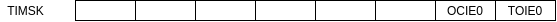
\includegraphics[width=320px]{images/18_Timer/TIMSK.png}
\end{figure}
\begin{itemize}
    \item TOIE0: abilita l' interruzione al wrap
    \item OCIE0: abilita l' interruzione sul match
\end{itemize}
I bit di flag invece si trovano in TIFR:
\begin{figure}[H]
    \centering
    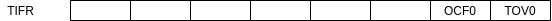
\includegraphics[width=320px]{images/18_Timer/TIFR.png}
\end{figure}
\begin{itemize}
    \item OCF0: flag dell' interrupt sul match
    \item TOV0: flag dell' interrupt sul wrap
\end{itemize}

\subsubsection{Esempio: orologio di sistema}
Inseriamo il prescaler massimo , quindi ad ogni wrap interrupt saranno passati $256 \cdot 1024 = 2^{18}$ cicli di clock, supponendo che $T_{ck} = 1\mu s$ ad ogni interrupt saranno passato $2^{18}\mu s$.
Ogni milione di cicli di clock invece è passato 1 secondo, quindi quando scatta l' interruzione aggiorno un contatore, e se è passato oltre 1M scalo 1M ed aggiorno il valore della variabile secondi, e così via per il resto. 


\subsection{Timer 1}
E' un timer a 16 bit quindi possiamo aspettare tempi più lunghi con un prescaler minore, abbiamo una risoluzione maggiore.
Essendo a 16 bit ogni registro di utilità è in realtà composto da due registri:
\begin{figure}[H]
    \centering
    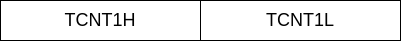
\includegraphics[width=200px]{images/18_Timer/TCNT1.png}
\end{figure}

\subsubsection{Comparatore}
Abbiamo due registri di comparazione:
\begin{figure}[H]
    \centering
    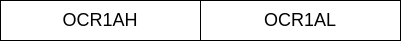
\includegraphics[width=200px]{images/18_Timer/OCR1A.png}
\end{figure}
\begin{figure}[H]
    \centering
    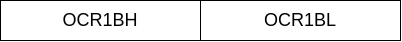
\includegraphics[width=200px]{images/18_Timer/OCR1B.png}
\end{figure}
tuttavia il reset al match può essere configurato solo per OCR1A quindi se si devono usare entrambi i comparatori conviene inserire valori tali che OCR1B $<$ OCR1A in quanto altrimenti il primo match resetta il contatore ed il secondo match non si avrà mai!

Abbiamo due pin di uscita da poter modificare al match: OC1A ed OC1B associati ad OCR1A ed OCR1B.
Abbiamo ovviamente due bit di controllo per ogni OCR1.

\subsubsection{Trigger esterno}
Nel package esiste un pin ICP1 (Input Capture Pin) ed il registro ICR1H/L:
\begin{figure}[H]
    \centering
    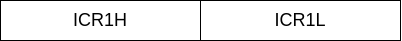
\includegraphics[width=200px]{images/18_Timer/ICR1.png}
\end{figure}
quando arriva un impulso sul pin ICP si copia il valore di TCNT1 in ICR1.
Possiamo implementare una specie di photofinish.

Si noti che è previsto anche che ICR1 possa essere usato come registro di match.

Es: con 16MHz di clock abbiamo una risoluzione di $T_R = 62,5 ns$, la velocità del suono è $V_{suono} = 340 \frac{m}{s}$ quindi la distanza percorsa in ogni istante misurato dal timer è di:
$d = 340 \times 62,5 \times 10^{-9} = 21,25 \mu m$
Possiamo misurare la distanza con una risoluzione di $21,25\mu m$ usando un radar sonoro.

\subsubsection{Cancellazione del rumore}
Attaccato al pin ICP1 c'è un circuito per la cancellazione del rumore:
\begin{figure}[H]
    \centering
    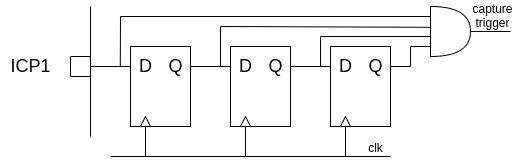
\includegraphics[width=250px]{images/18_Timer/noise_reduction_circuit.png}
\end{figure}
tengo in memoria il valore del pin ICP negli ultimi 4 clock, se è sempre stato ad 1 la porta AND lo rileva e scatta il trigger.

Questo circuito può essere utile ad esempio quando abbiamo inserito un interruttore meccanico per triggerare il pin ICP1, può succedere che in fase di chiusura non ci sia una transisione netta dal livello logico 0 al livello logico 1, piuttosto degli spike, sono dette \emph{alee}. Con questo circuito limitiamo enormemente il loro impatto.
E' anche detto \emph{debouncing} hardware, questo aggiunge un ritardo di 4 clock.
il valore della AND è poi inserito in un multiplexer per poter scegliere se triggerare la cattura del contatore sul livello logico basso o sul livello logico alto.

\subsubsection{Letture e scritture atomiche}
Essendo il contatore locato su due indirizzi per leggere dobbiamo eseguire due letture distinte, se lo facciamo mentre il timer corre potremmo avere dei problemi:
\begin{itemize}
    \item valore timer: 0x00FF, leggo la parte bassa ed ottengo 0xFF
    \item il clock incrementa il timer
    \item valore timer: 0x0100, leggo la parte superiore ed ottengo 0x01
    \item ho quindi letto 0x01FF, ho un errore enorme sul reale valore del timer
\end{itemize}
oppure:
\begin{itemize}
    \item valore timer: 0x00FF, leggo la parte alta ed ottengo 0x00
    \item il clock incrementa il timer
    \item valore timer: 0x0100, leggo la parte inferiore ed ottengo 0x00
    \item ho quindi letto 0x0000, anche qui un grande errore
\end{itemize}

Servirebbe poter leggere due indirizzi nello stesso ciclo di clock ma non possiamo farlo.
Per fortuna l'hardware del timer ci viene in aiuto:
\begin{figure}[H]
    \centering
    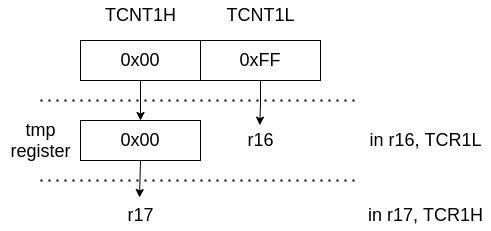
\includegraphics[width=250px]{images/18_Timer/atomic_read.png}
\end{figure}
\begin{itemize}
    \item nella prima lettura leggo direttamente la parte bassa che mi viene copiata nel registro r16, sempre durante questa lettura la parte alta viene letta ed inserita automaticamente in un registro temporaneo
    \item eseguendo la lettura della parte alta in realtà mi viene consegnato il valore inserito nel registro temporaneo
\end{itemize}
in questo modo ho ottenuto una lettura atomica.

Questa procedura è eseguita automaticamente per ogni registro a 16 bit della periferica quindi: \emph{per leggere un registro a 16 bit si deve prima leggere la parte bassa e poi la parte alta}, fare il contrario fornisce sicuramente risultati sbagliati.
Inoltre non si deve mai interrompere una lettura, se leggo il byte basso di qualche registro devo poi leggere anche la parte alta.

Si noti che continuano ad esserci problemi se entrano in gioco anche le interruzioni: ad esempio se leggo la parte bassa, e quindi l' alta mi viene messa nel registro temporaneo, ma poi parte una interruzione che legge i registri del timer, allora il registro temporaneo sarà stato sporcato e quindi la successiva lettura sarà sbagliata.

\emph{Le scritture vanno eseguite in maniera big endian cioè prima va scritta la parte alta, che verrà inserita nel registro temporaneo, e successivamente nella parte bassa}, solo a questo punto avviene la vera scrittura nel registro del timer.


\subsubsection{Configurazione}
I registri di controllo sono tutti su 8 bit e sono TCCR1A, TCCR1B, TCCR1C:
\begin{figure}[H]
    \centering
    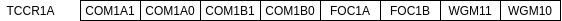
\includegraphics[width=320px]{images/18_Timer/TCCR1A.png}
\end{figure}
\begin{itemize}
    \item COM1Ax: indicano cosa fare al match con OCRA
    \item COM1Bx: indicano cosa fare al match con OCRB
    \item FOC1x: quando vengono settati lanciano un match parziale, quindi agiscono sul pin OC1A ed OC1B, ma senza lanciare l' interruzione
    \item WGM1x: indicano la modalità di funzionamento del timer
\end{itemize}

\begin{figure}[H]
    \centering
    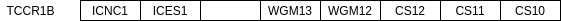
\includegraphics[width=320px]{images/18_Timer/TCCR1B.png}
\end{figure}
\begin{itemize}
    \item WGM1x: assieme ai bit WGM1x in TCCR1A configurano la modalità di funzionamento del timer
    \item ICNC1: abilita/disabilita la noise reduction
    \item ICES1: indica su quale fronte di ICP1 triggerarsi
    \item CS1x: selezionano il clock + prescaler da usare per aggiornare il contatore
\end{itemize}

\begin{figure}[H]
    \centering
    
\includegraphics[width=320px]{images/18_Timer/TIMSK_1.png}
\end{figure}
\begin{itemize}
    \item TICIE1: abilita l' interruzione sul cambiamento di valore sul pin ICP1
    \item OCIE1A: abilita l' interruzione sul match con OCRA
    \item OCIE1B: abilita l' interruzione sul match con OCRB
    \item TOIE1: abilita l' interruzione al wrap del timer
\end{itemize}

I bit di flag invece si trovano in TIFR:
\begin{figure}[H]
    \centering
    
\includegraphics[width=320px]{images/18_Timer/TIFR_1.png}
\end{figure}
\begin{itemize}
    \item ICF1: flag dell' interrupt sulla modifica del pin ICP1
    \item OCF1A: flag dell' interrupt sul match con OCR1A
    \item OCF1B: flag dell' interrupt sul match con OCR1A 
    \item TOV1: flag dell' interrupt sul wrap
\end{itemize}

\subsection{Timer 2}
Funziona come il timer 0, abbiamo quindi i registri:
\begin{itemize}
    \item TCNT2: registro contatore
    \item OCR2: registro di match 
    \item TCCR2: registro di controllo
\end{itemize}

Il timer 2 può essere usato in maniera asincrona cioè può essere aggiornato da un clock differente da quello della CPU.
In particolare è pensato per un oscillatore al quarzo per orologi (cioè a $2^{15}Hz$) inserito tra i pin TOSC1 e TOSC2 con lo stesso circuito visto per il clock generale.

Questa funzionalità è usata principalmente per poter staccare il clock originale e risparmiare energia dormendo per tempi più lunghi grazie alla bassa frequenza dell' oscillatore.

Es: ci risvegliamo dopo 255 conteggi ad una frequenza di $2^{15}Hz$ ed un prescaler di 1024. Si ha quindi una frequenza per l' aggiornamento del contatore di $\frac{2^{15}}{2^{10}} = 2^{5} = 32Hz$, per un wrap ci vogliono $\frac{256}{32Hz} = 8s$.

Dato che il clock di questo timer è asincrono potrebbe succedere di scrivere in uno dei suoi registri varie volte nello stesso ciclo di clock asincrono.
Questo è un problema in quanto renderebbe inconsistente qualsiasi scrittura che si sta eseguendo.

Per queste proprietà peculiari del timer esiste un registro di controllo a se:
\begin{figure}[H]
    \centering
    
\includegraphics[width=320px]{images/18_Timer/ASSR.png}
\end{figure}
\begin{itemize}
    \item AS2: abilita la modalità asincrona
    \item TCN2UB: quando è ad 1 indica che c'è già stata una scrittura su TCNT2 e quindi non si dovrebbe farne un' altra
    \item OCR2UB: quando è ad 1 indica che c'è già stata una scrittura su OCR2 e quindi non si dovrebbe farne un' altra
    \item TCR2UB: quando è ad 1 indica che c'è già stata una scrittura su TCCR2 e quindi non si dovrebbe farne un' altra
\end{itemize}
NB: UB sta per update busy, i bit busy vanno a 0 quando la scrittura è effettivamente avvenuta.


